\documentclass{standalone}
\usepackage{ tikz }

\begin{document}
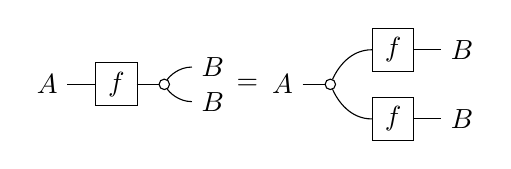
\begin{tikzpicture}[yscale=-1,x=1em,y=1.25em]
        
    \node [anchor=east] at (0,0) {$A$};
    \draw (0,0) -- (1,0);
    \node [draw, minimum width = 1.5em, anchor=west, fill=white] at (1,0) {$f$};
    \draw (2.5,0) -- (3.5,0);
    \node (C1) [draw, circle, fill=white, scale=0.4] at (3.5,0) {};
    \node (B1) [anchor=west] at (4.5,-0.5) {$B$};
    \node (B2) [anchor=west] at (4.5,0.5) {$B$};
    \draw (C1) to[out=285, in=180] (B1);
    \draw (C1) to[out=75, in=180] (B2); 

    \node at (6.5,0) {$=$};

    \node [anchor=east] at (8.5,0) {$A$};
    \draw (8.5,0) -- (9.5,0);
    \node (C2) [draw, circle, fill=white, scale=0.4] at (9.5,0) {};
    \node (F1) [draw, minimum width = 1.5em, anchor=west, fill=white] at (11,-1) {$f$};
    \node (F2) [draw, minimum width = 1.5em, anchor=west, fill=white] at (11,1) {$f$};
    \draw (C2) to[out=285, in=180] (F1);
    \draw (C2) to[out=75, in=180] (F2);
    \draw (12.5,-1) -- (13.5,-1);
    \draw (12.5,1) -- (13.5,1);
    \node [anchor=west] at (13.5,-1) {$B$};
    \node [anchor=west] at (13.5,1) {$B$};

\end{tikzpicture}
\end{document}